\subsection{Hyperbolische PDGL}
\begin{minipage}{14cm}
	PDGL: $\partFrac{^2u}{t^2}-a^2\partFrac{^2 u}{x^2}=0\qquad \Omega=\left\{(x,t)|t>0\right\}\qquad u_0=u(x_0,0)$\\
	
	Trick: $(\partial_t +a\partial_x)(\partial_t-a\partial_x)u=(\partial_t^2-a^2\partial_x^2)u=0$\qquad(für konstante Geschwindigkeit $a$)\\
	
	Zwei mögliche Lösungen: $\underset{\text{\cfbox{red}{Nach rechts laufende Welle}}}{\underbrace{(\partial_t +a\partial_x)u=0}}\qquad \underset{\text{\cfbox{black}{Nach links laufende Welle}}}{\underbrace{(\partial_t-a\partial_x)u=0}}$\\
	
	Lösung mittels Charakteristiken: $\partFrac{}{s}
	\begin{Bmatrix}
		x(s)\\
		t(s)\\
		u(s)
	\end{Bmatrix}=
	\begin{Bmatrix}
		\pm a\\
		1\\
		0
	\end{Bmatrix}
	\begin{array}{ll}
		\Rightarrow&x=\pm as +x_0\\
		\Rightarrow&t= s +t_0=s\qquad (t_0=0)\\
		\Rightarrow&u=u_0\\
	\end{array}
	$\\
	
	$x=\pm at+x_0\quad\Rightarrow\quad x_0=x\mp at\quad\Rightarrow\quad u(x,t)=u_0(x\mp at)$\\
	
	Allgemeine Lösung aus Linearkombination: $\boxed{u(x,t)=u_+(x+at)+u_-(x-at)}$\\
	
	$\Rightarrow$ Es werden \textbf{zwei} Anfangsbedingungen benötigt um $u_+$ \textbf{und} $u_-$ zu bestimmen.\\
	
	z.B.: $u(x,0)=u_0(x)\qquad \partFrac{u}{t}(x,0)=g_0(x)$
	\end{minipage}
	\hfill
	\begin{minipage}{5cm}
	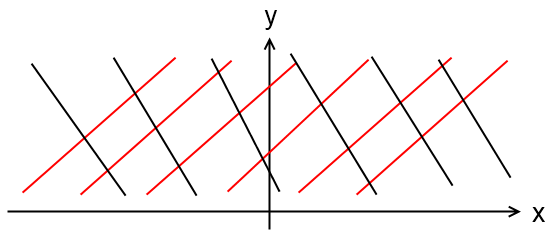
\includegraphics[width=5cm]{Content/01_theory/linksRechts}
	\end{minipage}
\subsubsection{Streifen/Charakteristiken}
	PDGL: $a\partial_x^2u+2b\partial_x\partial_yu+c\partial_y^2u+d\partial_xu+e\partial_yu+fu=g$ Symbolmatrix: $ 
		\begin{bmatrix}
			a & b\\
			b & c
		\end{bmatrix}$
	
	Entlang der Kurve $t\mapsto(x(t),y(t))$ sind die Anfangswerte / partiellen Ableitungen
	$
	\left.
	\begin{aligned}
	u(x(t),y(t))&=u(t)\\
	\partial_xu(x(t),y(t))&=p(t)\\
	\partial_yu(x(t),y(t))&=q(t)
	\end{aligned}
	\qquad
	\right\}
	\label{charanfangs}
	$
	
	Charakteristiken erfüllen DGL:
    \[
        a\dot y(t)^2-2b\dot x(t)\dot y(t)+c\dot x(t)^2=0
    \]
	
	Charakteristischer Streifen erfüllt zusätzlich: $a\dot p(t)\dot y(t)-h\dot x(t)\dot y(t)+c\dot x(t)\dot q(t)=0$